\chapter{Práctica 2}
En las practicas 0 y 1 trabajamos con las clases Fecha y Cadena, una vez implementadas correctamente
y funcionales vamos a trabajar con nuevas clases que haran uso de estas dos.

\begin{figure}[h]
    \begin{center}
        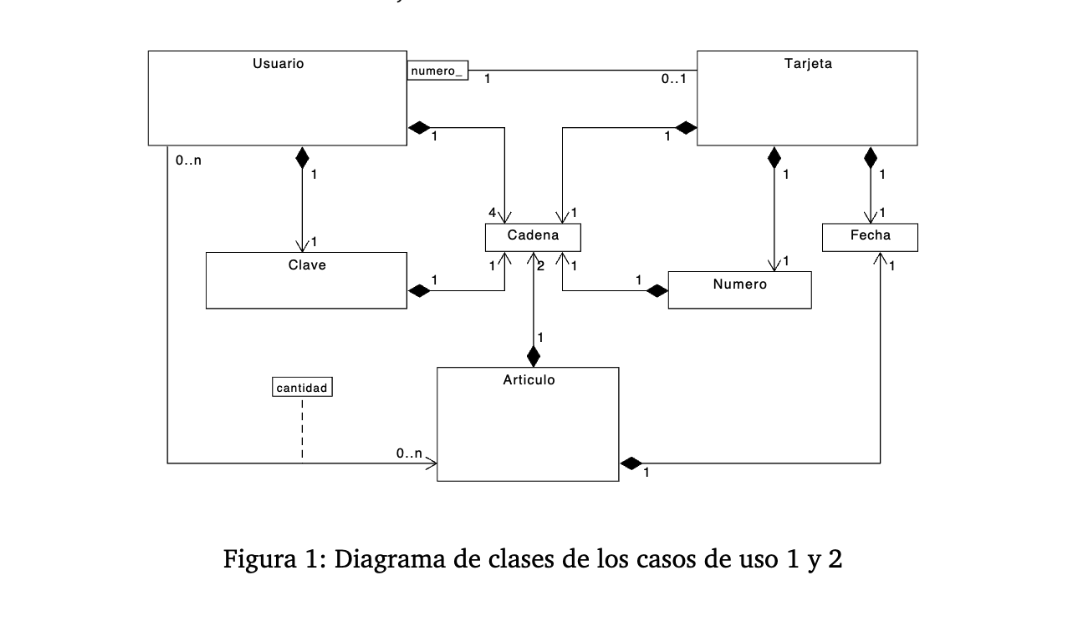
\includegraphics[width=\textwidth]{Pics/P2_1.png}
    \end{center}
\end{figure}
Mediante este diagrama vamos a crear las nuevas clases.
La clase Artículo irá en los ficheros articulo.[ch]pp. Las clases Usuario y Clave se 
escribirán en los ficheros usuario.[ch]pp. Las clases Tarjeta y Numero se escribirán en los 
ficheros tarjeta.[ch]pp.

\section{Clase Artículo}
    La clase Artículo contiene 5 atributos → código de referencia, título, fecha de publicación, 
precio y número de ejemplares a la venta. Los 3 primeros son no modificables.

Un objeto de la clase Artículo se construye mediante esos 5 atributos en el orden: 
referencia, título, fecha de publicación, precio y existencias.
Este último parámetro es opcional: si no se suministra, se toma como cero.

La clase Artículo tendrá los métodos observadores: \texttt{referencia()}, \texttt{titulo()},
 \texttt{f\_publi()},\\ \texttt{precio()} y \texttt{stock()}. 
 Estos dos últimos estarán sobrecargados para devolver una referencia al atributo correspondiente, con el fin de permitir su modificación.

Finalmente, contará con un operador de inserción en flujo (\texttt{<<}) que imprimirá los 
datos de un artículo con el formato:

\begin{center}
\texttt{"Fundamentos de C++", 1998. 29,95 €}
\end{center}

\subsection{Articulo.hpp}
\begin{minted}[breaklines]{C++}
#ifndef ARTICULO_HPP
#define ARTICULO_HPP

//Inclusión de librerías
#include "../P1/fecha.hpp"
#include "../P1/cadena.hpp"
#include <iostream>
#include <iomanip>
#include <locale.h>
class Articulo{
public:
    Articulo(Cadena referencia, Cadena titulo ,Fecha f_publi
    ,double precio,unsigned ejemplares =0):referencia_(referencia),titulo_(titulo),
    fpubli_(f_publi),precio_(precio),ejemplares_(ejemplares){}

    //Observadores de la clase
    inline const Cadena& referencia() const noexcept{return referencia_;}
    inline const Cadena& titulo()const noexcept{return titulo_;}
    inline const Fecha& f_publi()const noexcept{return fpubli_;}
    inline double precio()const noexcept{return precio_;}
    inline double& precio()noexcept{return precio_;}
    inline unsigned stock()const noexcept{return ejemplares_;}
    inline unsigned& stock()noexcept{return ejemplares_;}

private:
    const Cadena referencia_,titulo_;
    const Fecha fpubli_;
    double precio_;
    unsigned ejemplares_;
};

//Operador de inserción en flujo
std::ostream& operator <<(std::ostream& , const Articulo&)noexcept;
#endif // !ARTICULO_HPP 
\end{minted}
\newpage
\subsection{Articulo.cpp}
\begin{minted}[breaklines]{C++}
#include "articulo.hpp"

//Operador de inserción en flujo
std::ostream& operator <<(std::ostream& output, const Articulo& art)noexcept{
std::locale::global(std::locale(""));
output<<"["<<art.referencia()<<"] "<<"\""<<art.titulo()<<"\""<<", "
        <<art.f_publi().anno()<<". "
        <<std::fixed<<std::setprecision(2)<<art.precio()<<" €";
return output;
}
\end{minted}
\section{Clase Tarjeta y Número}
    Consta de dos clases \textbf{Numero} y \textbf{Tarjeta} las cuales ambas se definen en tarjeta.hpp y se implementan en tarjeta.cpp.

\subsection{Clase Numero}
Un Numero contendrá un atributo de tipo Cadena, ya que este «número» puede tener espacios de separación al principio, al final o, más normal, en medio.

Su constructor recibirá como parámetro esa Cadena con el número. Tendrá que quitarle los blancos y comprobar que es un número válido. Si no lo fuera lanzará la excepción \textbf{Numero::Incorrecto}.
Para saber si un dígito de dicho número es un caracter en blanco, recorreremos el número entero y mediante \texttt{isspace()}.

Dentro de la clase Numero vamos a declarar Razon con los elementos LONGITUD, DIGITOS y NO\_VALIDO, para representar por qué un Numero no es válido, y la clase Incorrecto, con un atributo de tipo \texttt{Numero::Razon}, el constructor que recibe una Razon como parámetro, y el método observador \textbf{razon()} que devuelve el atributo.

También contendrá un operadore de conversión a cadena de caracteres de bajo nivel, y deberá definirse el operador «menor que» para dos objetos de la clase.
\newpage
\subsection{Clase Tarjeta}
En la clase Tarjeta vamos a encontrar un tipo enum para indicar el tipo de la tarjeta, siendo las opciones: Otro, VISA, Mastercard, Maestro, JCB y AmericanExpress.

Tendrá varios atributos como:

\begin{itemize}
    \item Un Numero constante, que es el número de la tarjeta que viene troquelado,
    \item Un puntero a Usuario, que es el titular,
    \item Un Fecha constante, que es la de cadudidad,
    \item Un booleano que indicará si la Tarjeta está o no activa, siempre se crea activa.
\end{itemize}

La Tarjeta se construirá solamente a partir del Numero, el Usuario y la Fecha de cadudidad. Esta última es importante debido a que vamos a declarar la clase de excepción \textbf{Tarjeta::Caducada}.


Esta clase de excepción tendrá un atributo que almacena la fecha caducada, un constructor que la reciba como parámetro observador \texttt{cuando()}, que lo devolverá. 

En el constructor vamos a crear la asociación entre Tarjeta y Usuario mediante el método \texttt{es\_titular\_de()}.

También vamos a declara una clase de excepción \textbf{Tarjeta::Num\_Duplicado}, debido a que no pueden haber dos Tarjetas con el mismo número. Esta clase de excepción tiene un atributo que es el Numero, y un método observador \texttt{que()} que lo devuelve.

Vamos a eliminar tanto el \textbf{constructor de copia} como el \textbf{operador de asignación por copia}, debido a que no se puede crear una Tarjeta que tenga los mismo atributos que otra.

Vamos a tener varios métodos observador que van a devolver los atributos de la Tarjeta, estos métodos serán: \texttt{numero()}, \texttt{titular()}, \texttt{caducidad()} y \texttt{activa()}, este último se sobrecargará que recibirá el nuevo estádo de la Tarjeta en un parámetro booleano y devolverá dicho estado.

Además vamos a tener el método observador \texttt{tipo()} devolverá el Tipo de la Tarjeta. El tipo de Tarjeta estará determinado por los primeros dígitos del Numero que la contiene:
\begin{itemize}
    \item \textbf{AmericanExpress:} Los dos primeros dígitos del Numero son 34 ó 37.
    \item \textbf{JCB:} El primer dígito es 3 a excepción de 34 o 37.
    \item \textbf{VISA:} El primer dígito es 4.
    \item \textbf{Mastercard:} El primer dígito es 5.
    \item \textbf{Maestro:} El primer dígito es 6.
    \item \textbf{Otro:} El cualquier otro dígito.
\end{itemize}

Cuando se detruya un Usuario, como las tarjetas no se destruyen segurían ``vivas'' pero sin ningún titular asociado, por tanto, se llamará al método \texttt{anula\_titular()} que dará al puntero que representa al titular el valor nulo y desactivará la Tarjeta poniendo a \textbf{false} el atributo correspondiente, es decir, activa pasa a falso. El destructor de la clase Usuario llamará a este método para cada una de sus tarjetas.

A la hora de destruir una Tarjeta, en el destructor tenemos que eliminar la relación entre Tarjeta y Usuario, para ello llamamos al método \textbf{Usuario::no\_es\_titular\_de()} sobre su titular, en caso de que este no haya sido destruido previamente; de lo contrario, la Tarjeta habrá sido desligada de su Usuario al ser destruido este (vea el punto anterior).

Vamos a sobrecargar el operador de inserción en flujo \texttt{\textbf{operator <<}} para mostrar los atributos de la clase Tarjeta siguiendo el formato:

\begin{figure}[h]
    \begin{minipage}{0.4\textwidth}
            \texttt{tipo tarjeta}\\
            \texttt{ numero tarjeta}\\
            \texttt{titular facial}\\
            \texttt{Caduca: MM/AA}
    \end{minipage}
    \hfill
    \begin{minipage}{0.5\textwidth}
        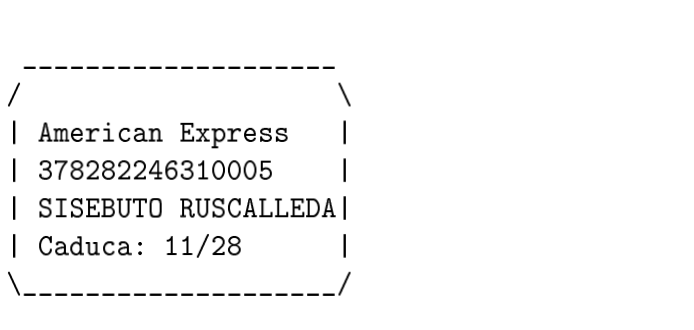
\includegraphics[width=\textwidth]{Pics/P2_2.png}
    \end{minipage}
    Donde MM es el mes de la fecha de caducidad, expresado con dos dígitos y AA son los dos últimos dígitos del año; por ejemplo: 11/28 sería noviembre de 2028.
    
    El titular facial es el nombre y apellido concatenados en mayúsculas del usuario titular de la tarjeta.

    Las lineas del formato no hace falta que las implementes, es más por estética.
\end{figure}
Para imprimir el nombre del tipo de la tarjeta (VISA, American Express...), deberá
sobrecargar también el operador de inserción para \textbf{Tarjeta::Tipo}, el cual imprimirá el texto «Tipo indeterminado» cuando el valor sea \textbf{Tipo::Otro}.

Dos Tarjeta podrán ordenarse por sus números. Para ello Tendrá que definir el operador menor-que de dos tarjetas.

\subsubsection{Tarjeta.hpp}
\begin{minted}[breaklines]{C++}
#ifndef TARJETA_HPP
#define TARJETA_HPP

//Inclusión de librerias
#include "../P1/fecha.hpp"
#include "../P1/cadena.hpp"
#include "usuario.hpp"
#include <iostream>
#include <set>
#include <algorithm> //remove_if
#include <cctype> //isspace
#include <cstring>
//declaraciones adelantadas
class Usuario;
class Clave;

/*-----Clase Numero-----*/
class Numero{
public:
    //tipos de excepciones
    typedef enum {LONGITUD,DIGITOS,NO_VALIDO}Razon;
    Numero(const Cadena&);
    
    //operador de conversion a const char*
    inline operator const char*()const{return numero_.operator const char *();}
    //sobrecarga del operador < para comparar numeros
    friend bool operator < (const Numero&, const Numero&);
    //clase de la excepcion
    class Incorrecto{
        Razon razon_;
        public:
            Incorrecto(const Razon& r):razon_(r){};
            const Razon& razon()const{return razon_;}
    };

private:
    Cadena numero_;
    //metodos extras para el constructor
    Cadena eliminar_espacios(const Cadena&); //devuelve la cadena sin espacios
    Cadena longitud(const Cadena&); //comprueba la longitud de la cadena es correcta o no
};

/*-----Clase Tarjeta-----*/
class Tarjeta{
public:
    //tipos de tarjetas
    typedef enum {Otro,VISA,Mastercard,Maestro,JCB,AmericanExpress} Tipo;
    Tarjeta(const Numero&, Usuario&, const Fecha&);
    //no se pueden crear tarjetas por copia de otras
    Tarjeta(const Tarjeta&)=delete;
    Tarjeta operator =(const Tarjeta&)=delete;
    //Observadores de la clase
    const Numero& numero()const noexcept{return numero_;}
    const Usuario* titular()const noexcept{return titular_;}
    const Fecha& caducidad()const noexcept{return caducidad_;}
    bool activa()const noexcept{return activa_;}
    bool activa(bool estado) noexcept {activa_=estado;return activa_;}//version modificadora de la anterior
    Tipo tipo()const noexcept;

    //destructor de la clase
    ~Tarjeta();
    //Clase de la excepcion tarjeta caducada
    class Caducada{
        Fecha fecha_;
        public:
            Caducada(const Fecha fecha):fecha_(fecha){};
            const Fecha& cuando()const{return fecha_;}
    };
    //Clase de la excepcion tarjeta duplicada
    class Num_duplicado{
        Numero num_;
        public:
            Num_duplicado(const Numero& num):num_(num){};
            const Numero& que()const{return num_;}
    };
    //Clase de la excepcion tarjeta desactivada
    class Desactivada{};
private:
    const Numero numero_;
    Usuario* const titular_;
    const Fecha caducidad_;
    bool activa_;

    //método privado de la clase
    //hacemos que la clase usuario sea amiga para poder hacer uso de este método
    friend class Usuario;
    void anula_titular();

    //conjunto de tarjetas
    static std::set<Numero>tarjetas_;
};
std::ostream& operator <<(std::ostream&, const Tarjeta& )noexcept;
std::ostream& operator <<(std::ostream&, const Tarjeta::Tipo& )noexcept;
//sobrecarga del operador <, para ordenar tarjetas
bool operator <(const Tarjeta&,const Tarjeta&);
#endif // !TARJETA_HPP
\end{minted}

\subsubsection{Tarjeta.cpp}
\begin{minted}[breaklines]{C++}
#include "tarjeta.hpp"
//inicialización del conjunto estático de tarjetas
std::set<Numero> Tarjeta::tarjetas_;
//Hacemos uso del algoritmo de luhn para ver si el numero de la tarjeta es correcto o no
bool luhn(const Cadena& numero);
/*-----Clase Numero-----*/
Numero::Numero(const Cadena& numero):numero_(longitud(numero)){
    char caracteres[] = "abcdefghijklmnopqrstuvwxyzABCDEFGHIJKLMNOPQRSTUVWXYZ./";
    //Comprobamos que está en el rango de caracteres
    if(strcspn(numero_.operator const char *(),caracteres)<numero_.length())
        throw Incorrecto(Razon::DIGITOS);
    //comprobamos que sea correcto
    if(!luhn(numero_))throw Incorrecto(Razon::NO_VALIDO);
}
bool operator < (const Numero& a, const Numero& b){
    return strcmp(a,b)<0;
}

//metodos privados de la clase
Cadena Numero::eliminar_espacios(const Cadena& cadena){
    //creamos una cadena nueva como copia de la introducida
    Cadena aux(cadena);
    const char* original = cadena.operator const char *();
    int j =0;
    for(size_t i =0; i!=strlen(original); i++){
        if(!isspace(original[i])){
            aux[j++] = original[i];
        }
    }
    aux[j] = '\0';
    return Cadena(aux.operator const char *());
}
Cadena Numero::longitud(const Cadena& cadena){
    //creamos una cadena como copia de la introducida para calcular la longitud sin espacios
    Cadena aux = eliminar_espacios(cadena);
    if(aux.length()> 19 || aux.length() < 13 || aux.length() <= 0)
        throw Incorrecto(Razon::LONGITUD);
    return aux;
}

/*-----Clase Tarjeta-----*/
Tarjeta::Tarjeta(const Numero& numero,  Usuario& titular, const Fecha& caducidad):
    numero_(numero),titular_(&titular),caducidad_(caducidad),activa_(true){
    if(caducidad_ < Fecha())throw Caducada(caducidad_); //caducada¿?
    //Comprobamos que la tarjeta no está registrada
    if(!tarjetas_.insert(numero).second)throw Num_duplicado(numero);
    //No caducada y numero correcto -> se asigna al usuario
    titular_ -> es_titular_de(*this);
}
Tarjeta::Tipo Tarjeta::tipo()const noexcept{
    switch (numero_[0]){
    case '3':
        if(numero_[1]=='4' || numero_[1]=='7') return Tipo::AmericanExpress;
        else return Tipo::JCB;
        break;
    case '4': return Tipo::VISA; break;
    case '5': return Tipo::Mastercard; break;
    case '6': return Tipo::Maestro; break;
    default: return Tipo::Otro; break;
    }
}

Tarjeta::~Tarjeta(){
    //Para poder eliminar una tarjeta, primero debemos de desvincularla de su titular
    if(Usuario* user = const_cast<Usuario*>(titular_)) user->no_es_titular_de(*this);
    tarjetas_.erase(numero_); //eliminamos despues de desvincular
}

bool operator <(const Tarjeta& a,const Tarjeta& b){
    return a.numero() < b.numero();
}

std::ostream& operator <<(std::ostream& output, const Tarjeta& t)noexcept{
    //primero tenemos que concatenar el nombre y el apellido del titular
    Cadena nombre_apell = t.titular()->nombre() + " " + t.titular()->apellidos();
    //las tenemos que imprimir en mayusculas
    int i =0;
    while(nombre_apell[i]!='\0'){
        if(islower(nombre_apell[i]))
            nombre_apell[i]=toupper(nombre_apell[i]);
        i++;
    }
    output<<std::setw(2)<<std::setfill(' ')<<' '<<t.tipo()
    <<std::setw(2)<<std::setfill(' ')<<' '<<t.numero()<<"\n"
    <<std::setw(2)<<std::setfill(' ')<<' '<<nombre_apell<<"\n"
    <<std::setw(2)<<std::setfill(' ')<<' '<<"Caduca: "<<std::setfill('0')<<std::setw(2)<<t.caducidad().mes()
    <<"/"<<std::setw(2)<<(t.caducidad().anno() % 100)<<std::endl;
    return output;
}

std::ostream& operator <<(std::ostream&output, const Tarjeta::Tipo& tipo )noexcept{
    switch (tipo){
    case Tarjeta::Otro: output<<"Otro"<<std::endl; break;
    case Tarjeta::VISA: output<<"VISA"<<std::endl; break;
    case Tarjeta::Mastercard: output<<"Mastercard"<<std::endl;break;
    case Tarjeta::Maestro: output<<"Maestro"<<std::endl; break;
    case Tarjeta::JCB: output<<"JCB"<<std::endl; break;
    case Tarjeta::AmericanExpress: output<<"AmericanExpress"<<std::endl; break;
    default: output<<"Otra"<<std::endl;break;
    }
return output;
}
void Tarjeta::anula_titular(){
    (Usuario*&) titular_=nullptr;
    activa_=false;
}
\end{minted}
\newpage
\section{Clase Usuario y Clave}
    Consta de dos clases Clave y Usuario las cuales ambas se 
definen en usuario.hpp y se implementan en usuario.cpp, como hemos 
comentado anteriormente.
\subsection{Clase Clave}
Esta clase se va a crear mediante una Cadena que alojará una contraseña que cifraremos.
El constructor recibirá una cadena caracteres de bajo nivel \texttt{const char *} que contendrá la contraseña sin cifrar.
Declaramos las clases de excepción \textbf{Clave::Incorrecta} que devolverá la razón por la que se ha llevado a cabo la excepción serán (CORTA y ERROR\_CRYPT), esta clase de excepción devolverá el atributo correspondiente mediante el observador \texttt{razon()}.

Tendremos un observador llamado \texttt{clave()} que devuelve la contraseña cifrada almacenada.

Por último encontramos el método \texttt{verifica()} que recibirá como parámetro una cadena de caracteres de bajo nivel (contraseña sin cifrar) y devuelve un booleano si se corresponde con la contraseña almacenada, en este caso devuelve \textbf{true}, si no \textbf{false}.

\subsection{Clase Usuario}
La clase Usuario contrendrá estos atributos:
\begin{itemize}
    \item 4 Cadenas que serán: identificador, nombre, apellido y dirección (por este orden).
    \item Una contraseña que será de tipo Clave.
    \item Un diccionario de tarjetas público (\texttt{std::map<Numero,Tarjeta*>}), que se tiene que llamar Tarjetas.
    \item El contenido del carrito, que será un diccionario de artículos junto con la cantidad de los mismos (\texttt{std::unordered\_map<Articulo*,unsigned>}) que es público y se tiene que llamar Articulos.
\end{itemize}

El constructor recibirá 5 parámetros que son: identificador, nombre, apellido, dirección y clave.
Este constructor debe de comprobar que el Usuario se crea correctamente:
\begin{itemize}
    \item Comprueba que el identificador no esté repetido, si no se lanza la excepción \textbf{Usuario::Id\_duplicado}, que devuelve el atributo a través del observador \texttt{idd()}.
    \item Un Usuario NO puede crearse por copia a través de otro (ni constructor ni operador de asignción por copia.)
\end{itemize}

La clase tendrá varios métodos observadores: \texttt{id()}, \texttt{nombre()}, \texttt{apellido()}, \texttt{direccion()}, \texttt{tarjetas()} y \texttt{compra()}. No devolvemos la clave.

Como la clase Usuario y Tarjeta están relacionadas entre sí, vamos a declarar el método \texttt{es\_titular\_de()} y \texttt{no\_es\_titular\_de()} que recibe como parámetro la tarjeta y que se encargarán de crear y eliminar los enlaces de las clases.

A la hora de destruir una tarjeta primero la tenemos que desvincular de su titular, por eso llamará al método \textbf{Tarjeta::anula\_titular()}

La clase Usuario y Articulo se relacionan mediante una asociación undireccional mediante el método \texttt{compra()}, que será una sobrecarga del observador, pero este va a recibir dos parámetros (Articulo y cantidad). Si la cantidad que se introduce es 0, se elimina, si es mayor que 0, se añade al carrito.
Con este método sobrecargado podemos eliminar Articulos de la compra, pero también tenemos el método \texttt{vaciar\_carro()} que eliminará todos los artículos del carro.

Mediante el observador \texttt{n\_articulos()} devolvemos el número de articulos que contiene el carrito.

Vamos a sobrecargar el operdor de inserción en flujo \texttt{operator <<} para mostrar los datos del Usuario con el formato:

    \textit{identificador [clave cifrada] nombre apellidos}\\
    \textit{dirección}\\
    \textit{Tarjetas:}\\
    \textit{\textless lista de tarjetas\textgreater}


Por último, vamos a definir otro método \texttt{mostrar\_carro()} (externa a la clase), para mostrar el contenido del carro en el flujo de salida con el formato:
\begin{center}
    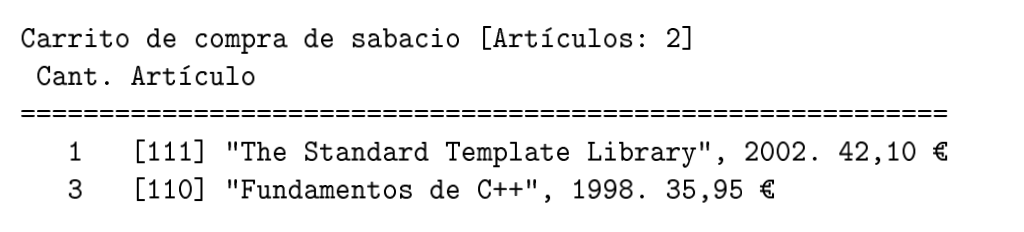
\includegraphics[width=\textwidth]{Pics/P2_3.png}
\end{center}

\newpage
\subsection{Usuario.hpp}
\begin{minted}[breaklines]{C++}
#ifndef USUARIO_HPP
#define USUARIO_HPP

//Inclusión de librerías
#include "../P1/cadena.hpp"
#include "tarjeta.hpp"
#include "articulo.hpp"
#include <random>
#include <map>
#include <unordered_map>
#include <unordered_set>
#include <iomanip>

//Declaraciones adelantadas
class Numero;
class Tarjeta;
/*-----Clase Clave-----*/
class Clave{
    public:
        typedef enum {CORTA,ERROR_CRYPT}Razon;
        Clave(const char*);

        //observador de la clase
        inline Cadena clave()const {return password_;}
        bool verifica(const char* )const;
        //Clase de la excepción
        class Incorrecta{
            Razon razon_;
            public:
                Incorrecta(const Razon& r):razon_(r){};
                const Razon& razon()const{return razon_;}
        };
    private:
        Cadena password_;
};

/*-----Clase Usuario-----*/
class Usuario{
    public:
        typedef std::map<Numero,Tarjeta*> Tarjetas;
        typedef std::unordered_map<Articulo*,unsigned int>Articulos;

        Usuario(const Cadena& ,const Cadena& , const Cadena& , const Cadena& , const Clave& );
        //eliminamos el ctor de copia y el operador de asignacion
        Usuario(const Usuario&)=delete;
        Usuario operator = (const Usuario&)=delete;
        //métodos observadores
        inline Cadena id()const noexcept{return identificador_;}
        inline Cadena nombre()const noexcept{return nombre_;}
        inline Cadena apellidos()const noexcept{return apellidos_;}
        inline Cadena direccion()const noexcept{return direccion_;}
        inline const Tarjetas& tarjetas()const noexcept{return tarjetas_;}
        inline const Articulos& compra()const noexcept{return articulos_;}
        
        //metodos de la asociacion con clase Tarjeta
        void es_titular_de(Tarjeta&) noexcept;
        void no_es_titular_de(Tarjeta&) noexcept;
        //métodos de la asociación unidireccional con Articulos
        void compra( Articulo&, size_t cantidad = 1) noexcept;
        inline void vaciar_carro() noexcept {articulos_.clear();}
        inline size_t n_articulos()const noexcept {return articulos_.size();}

        //destructor de la clase usuario
        ~Usuario();
        //Clase de la excepcion
        class Id_duplicado{
            Cadena id_;
            public:
                Id_duplicado(const Cadena& id):id_(id){};
                const Cadena& idd()const{return id_;}
        };
        friend std::ostream& operator <<(std::ostream& , const Usuario&)noexcept;
    private:
        const Cadena identificador_, nombre_,apellidos_,direccion_;
        Clave clave_;
        Tarjetas tarjetas_;
        Articulos articulos_;
        static std::unordered_set<Cadena> usuario_; //conjunto de usuarios no repetidos del programa
};
void mostrar_carro(std::ostream& , const Usuario&);
#endif // !USUARIO_HPP
    
    
\end{minted}

\subsection{Usuario.cpp}
\begin{minted}[breaklines]{C++}
#include "usuario.hpp"
#include <unistd.h> //crypt()

//Inicialización del conjunto global de usuarios
std::unordered_set<Cadena>Usuario::usuario_;
/*---Clase Clave----*/
Clave:: Clave(const char* c){
    //Comprobamos tamaño de la clave
    if(strlen(c)<5){
        throw Incorrecta(Razon::CORTA);
    }
    else{
        //Encriptamos la clave nueva
        const char* valores ="abcdefghijklmnopqrstuvwxyzABCDEFGHIJKLMNOPQRSTUVWXYZ0123456789./";
        std::random_device random;
        std::uniform_int_distribution<>distribucion(0,63);
        char cifrado[2]={valores[distribucion(random)],valores[distribucion(random)]};
        //comprabamos que el cifrado sea correcto, si no excepción
        if(crypt(c,cifrado)){
            password_ = crypt(c,cifrado);
        }else{
            throw Incorrecta(Razon::ERROR_CRYPT);
        }
    }
}
bool Clave::verifica(const char* clave)const{
    //compara la encriptación de la clave que hemos metido concuerda con una de las claves
    return !(strcmp(crypt(clave, password_.operator const char *()),
                password_.operator const char *()));
}

/*-----Clase Usuario-----*/
Usuario::Usuario(const Cadena& id ,const Cadena& nom, const Cadena& apell ,const Cadena& dir ,const Clave& clave):
    identificador_(id),nombre_(nom),apellidos_(apell),direccion_(dir),clave_(clave){
    //Vamos a compromar si el usuario no existe en la lista de usuarios del programa
    if(!usuario_.insert(id).second)throw Usuario::Id_duplicado(id);
}
void Usuario::es_titular_de(Tarjeta& t) noexcept{
    //asosicamos el usuario con la tarjeta
    if(this==t.titular()){
        tarjetas_.insert(std::make_pair(t.numero(),&t));
    }
}

void Usuario::no_es_titular_de(Tarjeta& t) noexcept{
    //desvinculamos el usuario con la tarjeta
    t.anula_titular();
    tarjetas_.erase(t.numero());
}

void Usuario::compra( Articulo& art, size_t cantidad) noexcept{
    //si la cantidad del articulo es > 0 -> se añade; si no se elimina
    if(cantidad > 0)articulos_[&art]=cantidad; //articulos_.insert(std::make_pair(&art,cantidad));
    else articulos_.erase(&art);
}

Usuario::~Usuario(){
    //Para eliminar al usuario tenemos que desligar todas sus tarjetas y luego
    //eliminarlo
    for(auto i = tarjetas_.begin(); i!=tarjetas_.end();i++){
        i->second->anula_titular();
    }
    usuario_.erase(identificador_);
}
    
void mostrar_carro(std::ostream& output , const Usuario& user){
    output << "Carrito de compra de "<<user.id()<<" [Artículos: "<<user.n_articulos()<<"]\n"
            << "Cant. Artículo"<<std::endl;
    output <<std::setw(95)<<std::setfill('=')<<' '<<std::endl; //estética del formato
    //creamos una variable para tener control del numero de articulos del carro
    int n_art = user.n_articulos();
    while(n_art > 0){
        for(auto i=user.compra().begin();i!=user.compra().end();i++){
            output<<std::setw(4)<<std::setfill(' ')<< i->second
                <<" ["<<(*i->first).referencia()<<"] "<<"\""
                <<(*i->first).titulo()<<"\""<<", "
                <<(*i->first).f_publi().anno()<<". "
                <<std::fixed<<std::setprecision(2)<<(*i->first).precio()<<" €"<<std::endl;
            n_art--;
        }
    }
}
std::ostream& operator <<(std::ostream& output , const Usuario& user)noexcept{
    output << user.id() <<" ["<<user.clave_.clave().operator const char *()<<"] "<<user.nombre()<<" "
    <<user.apellidos()<<"\n"<<user.direccion()<<std::endl;
    output<<"Tarjetas: \n"<<std::endl;
    for(auto i = user.tarjetas().begin(); i!=user.tarjetas().end(); i++)
        output<< *i->second<<std::endl;
    return output;
}
    
\end{minted}


